\section{Statistical procedure in full}
\label{app:stats}

\paragraph{Success rate.}
The primary test is the two-sided \emph{exact} McNemar (binomial) test on the
discordant counts, computed from the exact binomial tail rather than the
$\chi^2$ approximation, because the discordant counts here are small ($b+c \le
10$ per fault). We also report the mid-$p$ variant, which is less conservative at
these sizes, and the Haldane--Anscombe corrected matched odds ratio. Multiplicity
across the five faults is controlled by Holm--Bonferroni; Benjamini--Hochberg is
implemented and reported in the released code for comparison.

\paragraph{Intervals.}
Confidence intervals for $D(F)$ come from a percentile bootstrap that resamples
\emph{pair units} --- the correct resampling unit for a paired design, as opposed
to resampling trials, and the seed is fixed (\texttt{BootSeed}$=$\BootSeed{},
\BootIters{} resamples) so the interval is reproducible. Because a single
bootstrap seed can be selected to flatter a result, we also compute the interval
under five additional seeds and report the envelope in the released artifacts. We
additionally computed a task-clustered sensitivity interval, which is wider than
the pair-level interval when the same task is correlated across seeds; both are in
the released statistics files.

\paragraph{Process measures.}
Deltas in step count and wall-clock time are not binary, so we use the two-sided
Wilcoxon signed-rank test with the Hodges--Lehmann estimator of the shift; the
distributions are heavy-tailed and contain ties, which is why we do not report a
paired $t$-test. These tests are run on the behavioural matrix, which is
\emph{not} the same data as the official subset (\secref{sec:setup}).

\paragraph{Power.}
The minimum detectable effect for a paired proportion design is obtained by
solving

\begin{equation}
  n \;=\; \frac{\bigl(z_{1-\alpha/2}\sqrt{\pi_d}
        + z_{\text{power}}\sqrt{\pi_d - \delta^2}\bigr)^2}{\delta^2}
\end{equation}

for $\delta$, where $\pi_d = \mathbb{P}(\text{arms disagree})$. Two subtleties we
had to get right, and that we suspect are easy to get wrong: the risk difference
is bounded by $\pi_d$, not by $1$, so the search must be bracketed on
$(0, \pi_d]$; and when the bracket is wrong the equation silently returns
undefined rather than failing loudly. We use the \emph{observed} discordance
$\pi_d = \PiDNative{}$ rather than a round number, and we report cases where the
target power is unreachable at any effect size as \emph{undefined} rather than
quoting a number.

% GENERATED by scripts/paper/make_tables.py -- do not edit by hand.
\begin{table}[t]
\centering
\small
\caption{Minimum detectable paired difference in success rate (percentage points) at $\alpha=\Alpha{}$, power $\Power{}$. \textbf{n/a} means the design cannot reach the target power at \emph{any} effect size the paired design can express (the risk difference is bounded by $\pi_d$). The native-evaluator analysis has only $n=\ResWebDomMissingNNat$--$\ResWebTimeoutNNat$ pairs per fault. The $n=40$ column is therefore a counterfactual, and a null result under the actual design cannot be read as evidence of robustness.}
\label{tab:power}
\begin{adjustbox}{max width=\linewidth}
\begin{tabular}{lrrrr}
\toprule
Discordance $\pi_d$ & MDE at $n=31$ & MDE at $n=40$ & MDE at $n=80$ & MDE at $n=155$ \\
\midrule
0.10 & n/a & n/a & 9.8 & 7.1 \\
0.15 & n/a & n/a & 12.0 & 8.6 \\
0.20 & n/a & 19.2 & 13.8 & 10.0 \\
0.25 & 24.2 & 21.5 & 15.4 & 11.2 \\
0.30 & 26.5 & 23.6 & 16.9 & 12.2 \\
\bottomrule
\end{tabular}
\end{adjustbox}
\end{table}


\section{Pooled-evaluator table}
\label{app:pooled}

For completeness, Table~\ref{tab:official_all} reports the same analysis with the
evaluator paths pooled. It is not a robustness result and we do not use it as one;
we include it to show how much the conclusion moves when the fallback
contamination is left in, and to demonstrate why any published number of this form
should be accompanied by its stratified version.

% GENERATED by scripts/paper/make_tables.py -- do not edit by hand.
\begin{table}[t]
\centering
\small
\caption{Primary fault result, \emph{all} evaluator paths pooled. Reported for completeness; the fallback adapter is structurally failure-biased (see Table~\ref{tab:official_native}).}
\label{tab:official_all}
\begin{adjustbox}{max width=\linewidth}
\begin{tabular}{lrrrrrrrrrr}
\toprule
Fault & $n$ & Disc. & Control & Fault & $\Delta$ (pp) & 95\% CI (pp) & $p_{\text{exact}}$ & $p_{\text{mid}}$ & $p_{\text{Holm}}$ & OR \\
\midrule
DOM omission & 40 & 15 & 67.5\% & 65.0\% & $-$2.5 & [$-$22.5, $+$17.5] & 1.000 & 0.804 & 1.000 & 0.88 \\
Popup block & 40 & 11 & 57.5\% & 60.0\% & $+$2.5 & [$-$12.5, $+$17.5] & 1.000 & 0.774 & 1.000 & 1.18 \\
HTTP error & 40 & 12 & 57.5\% & 62.5\% & $+$5.0 & [$-$12.5, $+$22.5] & 0.774 & 0.581 & 1.000 & 1.36 \\
Timeout & 40 & 6 & 65.0\% & 65.0\% & $+$0.0 & [$-$12.5, $+$12.5] & 1.000 & 1.000 & 1.000 & 1.00 \\
Parameter error & 40 & 8 & 77.5\% & 62.5\% & $-$15.0 & [$-$27.5, $-$2.5] & 0.070 & 0.039 & 0.352 & 0.20 \\
\textbf{All faults} & 200 & 52 & 65.0\% & 63.0\% & $-$2.0 & [$-$9.0, $+$5.0] & 0.678 & 0.583 & 1.000 & 0.86 \\
\bottomrule
\end{tabular}
\end{adjustbox}
\vspace{2pt}
\parbox{\linewidth}{\footnotesize $\Delta$ is the paired risk difference (fault $-$ control); the interval is a percentile bootstrap over pair units and is descriptive --- the exact McNemar $p$ is the primary inferential quantity. OR is the Haldane-corrected matched odds ratio.}
\end{table}


\section{Architecture pilot table}
\label{app:arch}

Table~\ref{tab:architecture} gives the raw architecture pilot discussed in
\secref{sec:res-arch}. Rows are broken out by fault rather than by the artifact's
coarse \texttt{condition} column, which pools two different faults into one
bucket.

% GENERATED by scripts/paper/make_tables.py -- do not edit by hand.
\begin{table}[t]
\centering
\small
\caption{Architecture comparison --- \textbf{PILOT, $n=9$ per cell}. Rows are broken out by fault; \emph{not} by the artifact's coarse \texttt{condition} column, which pools the 2 injected faults into a single 18-row bucket. The committed \texttt{run\_architecture\_matrix.py} does not reproduce these 54 rows (different task set and seed range), so this table supports no architecture ranking. The two architectures also differ sharply in wall-clock (\ArchReactTime{}~s vs \ArchPlanTime{}~s on the control arm), which confounds any equal-budget comparison; the artifact records no per-role call counters, so budget equality cannot be verified.}
\label{tab:architecture}
\begin{adjustbox}{max width=\linewidth}
\begin{tabular}{lrrrrrrr}
\toprule
Architecture & Condition & $n$ & Success & Rate & Steps & LLM calls & Time (s) \\
\midrule
plan\_execute & none (control) & 9 & 0/9 & 0.0\% & 3.11 & 6.89 & 364.8 \\
plan\_execute & web\_dom\_missing & 9 & 1/9 & 11.1\% & 4.22 & 4.22 & 516.4 \\
plan\_execute & web\_http\_error & 9 & 1/9 & 11.1\% & 5.22 & 5.22 & 788.5 \\
react & none (control) & 9 & 4/9 & 44.4\% & 5.00 & 5.00 & 77.4 \\
react & web\_dom\_missing & 9 & 4/9 & 44.4\% & 4.89 & 4.89 & 82.6 \\
react & web\_http\_error & 9 & 3/9 & 33.3\% & 8.00 & 8.00 & 218.9 \\
\bottomrule
\end{tabular}
\end{adjustbox}
\end{table}


\section{The recovery artifact in full}
\label{app:recovery}

The recovery artifact records behavioural flags --- whether the observation was
refreshed, whether the tool changed, whether a stale action was repeated --- which
is exactly the process-level evidence one would want for attribution. In practice
\RecDegenerateCount{} of its columns are constant across all \RecN{} rows and
carry no information; \texttt{plan\_revised} was never recorded at all; and
\texttt{recovered} is row-for-row identical to \texttt{official\_success}, so it
is not an independent measurement of recovery but a restatement of the outcome it
would be used to explain. The \texttt{behavior\_labels} column is a deterministic
function of \texttt{recovered} (recovered $\Rightarrow$
\texttt{observation\_refreshed}, otherwise \texttt{fault\_detected}), so
correlations between the two are tautological. Two further columns are the same
predicate under different names (\texttt{stale\_action\_repeated} and
\texttt{retry}), and \texttt{fault\_detected} is recorded only on the
not-recovered subset, so it is computed over a different denominator from the
rest of the table.

We report the table rather than silently dropping it because the failure mode is
instructive: a recovery-behaviour artifact can look rich --- a dozen behavioural
columns --- while containing two varying quantities, one of which is the outcome.
Process-level attribution needs columns that vary \emph{independently} of the
outcome, and that has to be checked before the analysis, not after.

% GENERATED by scripts/paper/make_tables.py -- do not edit by hand.
\begin{table}[t]
\centering
\small
\caption{The recovery artifact on its 45-trial subset. It is \textbf{degenerate}: \texttt{observation\_after\_fault}, \texttt{plan\_revised}, \texttt{premature\_stop}, \texttt{retry\_executed}, \texttt{stale\_action\_repeated}, \texttt{tool\_changed} are constant across all 45 rows and therefore carry no information; \texttt{plan\_revised} was never recorded (empty, not false); and \texttt{recovered} is row-for-row identical to \texttt{official\_success}. \texttt{behavior\_labels} is a deterministic function of \texttt{recovered} (recovered $\Rightarrow$ \texttt{observation\_refreshed}, otherwise \texttt{fault\_detected}), not an independent observation. Only the columns shown vary.}
\label{tab:recovery}
\begin{adjustbox}{max width=\linewidth}
\begin{tabular}{lrrrr}
\toprule
Fault & $n$ & Official success & Rate & \texttt{goto\_fallback} \\
\midrule
Parameter error & 9 & 8/9 & 88.9\% & 0/9 \\
DOM omission & 9 & 7/9 & 77.8\% & 0/9 \\
HTTP error & 9 & 6/9 & 66.7\% & 2/9 \\
Popup block & 9 & 8/9 & 88.9\% & 0/9 \\
Timeout & 9 & 7/9 & 77.8\% & 0/9 \\
\textbf{All faults} & 45 & 36/45 & 80.0\% & 2/45 \\
\bottomrule
\end{tabular}
\end{adjustbox}
\end{table}


\section{Reproducibility of the runs}
\label{app:runs}

Every trial records its fault seed, injection step, model profile, architecture,
and git commit. The provider does not guarantee bit-identical sampling for a fixed
seed, so our reproducibility claim is at the level of the design (same fault, same
step, same task/seed pairing) rather than the token sequence; we state this
explicitly rather than claiming seed determinism we cannot verify. Wall-clock is
host- and load-dependent, which is why process-cost claims are made on within-pair
deltas only --- the five per-fault control arms are the \emph{same} configuration
yet differ by a factor of \NoiseFloorRatio{} in mean wall-clock
(\NoiseFloorLo--\NoiseFloorHi{}~s), so cross-arm absolute timings are dominated by
machine-level drift and are not interpretable.

\section{Candidate repairs and what an ablation would need}
\label{app:repair}

Four policy changes follow from the mechanisms in \secref{sec:repair}: error-aware
retry with backoff instead of re-deriving the whole plan; argument validation
against the current observation before dispatch; stale-observation detection that
forces a re-observation; and a termination policy for unobservable state. The last
is a judgement call rather than an automatic improvement --- the DOM-omission and
popup arms are \emph{faster} than control (\BehWebDomMissingTimeDelta{}~s and
\BehWebPopupBlockTimeDelta{}~s), which we read as early termination, so the
objective could be either to shorten that path further or to have the agent report
the blockage instead of silently failing. Each is testable in the existing harness
by running the same paired design with the repair enabled in both arms. None has
been run.

One fix \emph{was} made during this work --- correcting the task schema and
completion check, and detecting the compatibility fallback contaminating the
evaluator (\secref{sec:fallback}) --- and it must be classified correctly: it
raises the measured success rate by up to \BaselineSwing{}~pp, more than any fault
effect in this paper, and it improves the \emph{measurement}, not the \emph{agent}.
Reporting it as a robustness improvement would be precisely the error this paper is
about; any web-agent robustness claim drawn from a pipeline with a fallback path, a
schema mismatch, or an unvalidated completion check is measuring the harness.

A credible before/after comparison would therefore need to (i)~re-use the paired
design and the native-only stratum, (ii)~be sized against \secref{sec:res-power}
rather than against available compute --- at the observed discordance a $10$~pp
success-rate improvement needs roughly \PairsForTenPPObserved{} pairs per arm, so a
process-cost improvement is the realistic target at smaller $n$ --- and (iii)~run
the repaired arm concurrently with the unrepaired one, so that machine-level drift,
which spans a factor of \NoiseFloorRatio{} across nominally identical arms, does
not masquerade as an effect.

\section{Graphical summaries}
\label{app:figs}

Figures~\ref{fig:forest}, \ref{fig:behavior} and \ref{fig:noisefloor} show the
three quantitative summaries in graphical form. They are generated by the same
command as the tables, from the same statistics, so they cannot drift from them.

% GENERATED by scripts/paper/figures.py -- do not edit by hand.
\begin{figure}[t]
\centering
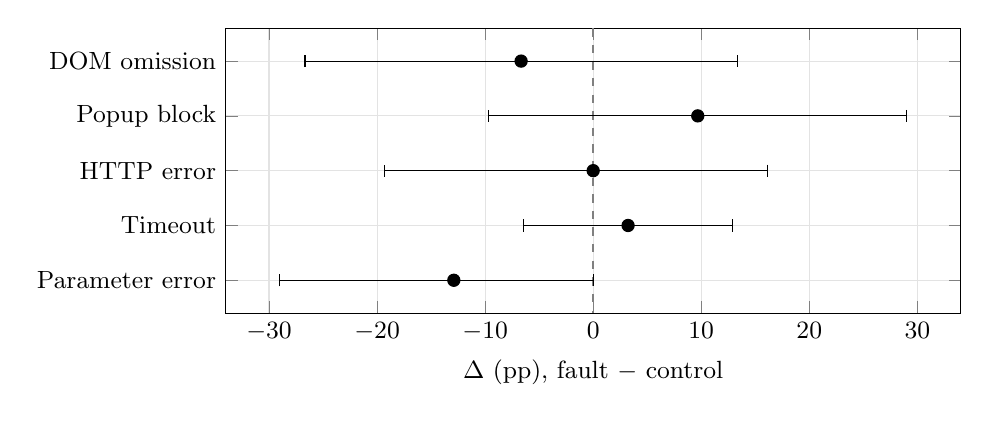
\begin{tikzpicture}
\begin{axis}[
  width=0.9\linewidth, height=5.2cm,
  xlabel={$\Delta$ (pp), fault $-$ control},
  ytick={1,2,3,4,5}, yticklabels={{DOM omission},{Popup block},{HTTP error},{Timeout},{Parameter error}},
  y dir=reverse, ymin=0.4, ymax=5.6,
  xmin=-34, xmax=34, xtick={-30,-20,-10,0,10,20,30},
  grid=major, grid style={gray!22},
  tick label style={font=\small}, label style={font=\small},
]
\draw[gray,dashed,thick] (axis cs:0,0.4) -- (axis cs:0,5.6);
\addplot[only marks, mark=*, mark size=2.2pt, black,
  error bars/.cd, x dir=both, x explicit]
  coordinates {(-6.67,1) -= (20.00,0) += (20.00,0) (9.68,2) -= (19.35,0) += (19.35,0) (0.00,3) -= (19.35,0) += (16.13,0) (3.23,4) -= (9.68,0) += (9.68,0) (-12.90,5) -= (16.13,0) += (12.90,0)};
\end{axis}
\end{tikzpicture}
\caption{Paired risk difference $\Delta$ in official success (fault $-$ control) on native-evaluator pairs, with the percentile bootstrap interval over pair units. Every interval spans zero and no fault survives Holm correction, which is the paper's primary result. Compare Table~\ref{tab:official_native}.}
\label{fig:forest}
\end{figure}

% GENERATED by scripts/paper/figures.py -- do not edit by hand.
\begin{figure}[t]
\centering
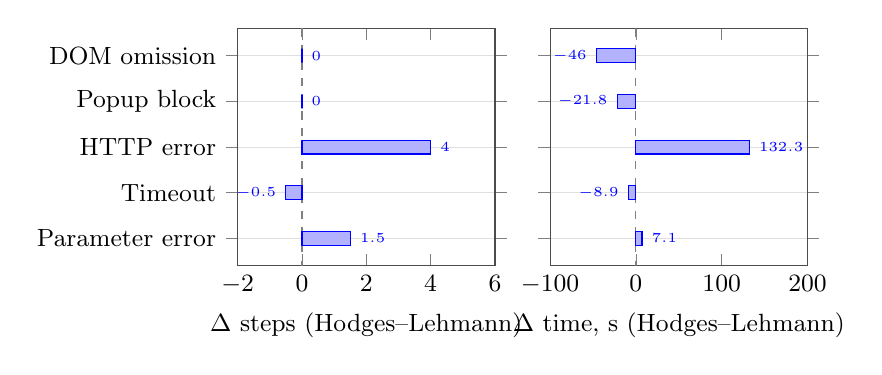
\begin{tikzpicture}
\begin{axis}[name=steps, xbar, bar width=5pt,
  width=0.40\linewidth, xmin=-2, xmax=6,
  ytick={1,2,3,4,5}, y dir=reverse, ymin=0.4, ymax=5.6,
  height=4.6cm,
  tick label style={font=\small}, label style={font=\small},
  nodes near coords, nodes near coords style={font=\tiny},
  ymajorgrids, grid style={gray!25},
  yticklabels={{DOM omission},{Popup block},{HTTP error},{Timeout},{Parameter error}},
  xlabel={$\Delta$ steps (Hodges--Lehmann)},
  fill=gray!60, draw=black!70,
]
\draw[gray,dashed] (axis cs:0,0.4) -- (axis cs:0,5.6);
\addplot coordinates {(0.0,1) (0.0,2) (4.0,3) (-0.5,4) (1.5,5)};
\end{axis}
\begin{axis}[name=time, at={(steps.east)}, anchor=west, xshift=0.7cm,
  xbar, bar width=5pt, width=0.40\linewidth, xmin=-100, xmax=200,
  ytick={1,2,3,4,5}, y dir=reverse, ymin=0.4, ymax=5.6,
  height=4.6cm,
  tick label style={font=\small}, label style={font=\small},
  nodes near coords, nodes near coords style={font=\tiny},
  ymajorgrids, grid style={gray!25},
  yticklabels={},
  xlabel={$\Delta$ time, s (Hodges--Lehmann)},
  fill=gray!60, draw=black!70,
]
\draw[gray,dashed] (axis cs:0,0.4) -- (axis cs:0,5.6);
\addplot coordinates {(-46.0,1) (-21.8,2) (132.3,3) (-8.9,4) (7.1,5)};
\end{axis}
\end{tikzpicture}
\caption{Within-pair process cost on the behavioural matrix. HTTP errors and parameter errors cost the agent steps and time, while DOM omission and popup blocking make it \emph{faster} --- which we read as fault-induced early termination. All five are significant at $p<0.01$ except where noted in Table~\ref{tab:behavior}.}
\label{fig:behavior}
\end{figure}

% GENERATED by scripts/paper/figures.py -- do not edit by hand.
\begin{figure}[t]
\centering
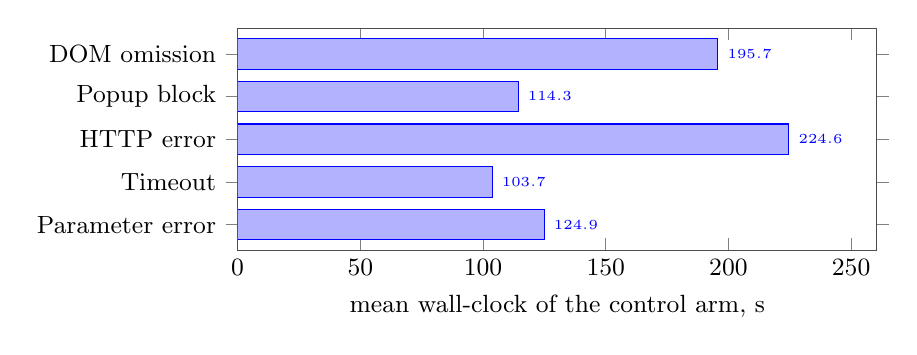
\begin{tikzpicture}
\begin{axis}[
  width=0.8\linewidth, height=4.4cm,
  xbar, bar width=11pt, xmin=0, xmax=260.5,
  ytick={1,2,3,4,5}, y dir=reverse, ymin=0.4, ymax=5.6,
  yticklabels={{DOM omission},{Popup block},{HTTP error},{Timeout},{Parameter error}},
  xlabel={mean wall-clock of the control arm, s},
  tick label style={font=\small}, label style={font=\small},
  nodes near coords, nodes near coords style={font=\tiny},
  fill=gray!55, draw=black!70,
]
\addplot coordinates {(195.7,1) (114.3,2) (224.6,3) (103.7,4) (124.9,5)};
\end{axis}
\end{tikzpicture}
\caption{The noise floor. These five arms are the \emph{same} agent configuration under the clean condition; each is the control half of one fault's pair set. Their means span a factor of 2.17$\times$, so absolute cross-arm timings are dominated by machine-level drift and only within-pair deltas are interpretable.}
\label{fig:noisefloor}
\end{figure}


\section{Supplementary experiment plan}
\label{app:plan}

The staged design that would make the attribution question answerable is released
with this paper. It is ordered by its ability to change the numbers reported here,
not by novelty. \textbf{Stage A} first repairs the evaluator's null-retrieval
schema path and re-evaluates the existing 400 response/HAR pairs offline. Every
frozen row already retains HAR, so repeating the same agent trials would not
remove the schema-triggered fallback; new runs are needed only for artifacts that
the repaired evaluator cannot consume or for deliberately replaced tasks.
\textbf{Stage C} crosses three categorical model levels with three architectures
and three faults. We do not impose an ordinal model-capability contrast: current
provider claims invalidate the earlier Flash--Pro ordering, and the cross-provider
ordering is not independently identified. The confirmatory target is therefore
the omnibus model$\times$architecture interaction followed by preregistered
pairwise and simple-effect contrasts.
\textbf{Stages E and F} add injection-step sensitivity and the repair ablation,
respectively; the former Stage B and D expansions are folded into Stage C. Injection-step sensitivity is
the confound we would press on hardest as a reviewer, since our injector holds the
step fixed throughout. The plan gives exact command lines, the six-worker
wall-clock budget measured from the runs reported here, and the per-trial timings
that size each stage.
